% Harus dimuat terlebih dahulu, digunakan agar file PDF memiliki format karakter yang benar.
% Untuk informasi lebih lanjut, lihat https://ctan.org/pkg/cmap.
\RequirePackage{cmap}

% Format dokumen sebagai paper konferensi menggunakan aturan IEEEtran terbaru (v1.8b).
% Untuk informasi lebih lanjut, lihat http://www.michaelshell.org/tex/ieeetran/.
\documentclass[conference]{IEEEtran}

% Format encoding font dan input menjadi 8-bit UTF-8.
\usepackage[T1]{fontenc}
\usepackage[utf8]{inputenc}
\usepackage{amsmath}
% Digunakan untuk mengatur margin dokumen.
\usepackage{textcomp}
\usepackage{float}

% Digunakan untuk tujuan demonstrasi.
\usepackage{mwe}

% Digunakan untuk menampilkan font dengan style yang lebih baik.
\usepackage[zerostyle=b,scaled=.75]{newtxtt}

% Digunakan untuk menampilkan tabel dengan style yang lebih baik.
\usepackage{booktabs}
\usepackage[table,xcdraw]{xcolor}

% Digunakan untuk menampilkan gambar pada dokumen.
\usepackage{graphicx}

% Digunakan untuk menampilkan potongan kode.
\usepackage{listings}
\lstset{
  basicstyle=\ttfamily,
  columns=fixed,
  basewidth=.5em,
  xleftmargin=0.5cm,
  captionpos=b
}

\usepackage{tabularx}
\usepackage{wrapfig}
% Digunakan agar backticks (`) dapat dirender pada PDF.
% Untuk informasi lebih lanjut, lihat https://tex.stackexchange.com/a/341057/9075.
\usepackage{upquote}

% Digunakan untuk menyeimbangkan bagian akhir dokumen dengan dua kolom.
\usepackage{balance}

% Digunakan untuk menampilkan pustaka.
\usepackage[square,comma,numbers,sort&compress]{natbib}

% Mengubah format ukuran teks pada natbib.
\renewcommand{\bibfont}{\normalfont\footnotesize}

% Jika melebihi 3 penulis dapat dilakukan linebreakend 
\makeatletter
\newcommand{\linebreakand}{%
  \end{@IEEEauthorhalign}
  \hfill\mbox{}\par
  \mbox{}\hfill\begin{@IEEEauthorhalign}
}
\makeatother

% Menambah nama penulis ketika menggunakan perintah \citet.
% Untuk informasi lebih lanjut, lihat https://tex.stackexchange.com/a/76075/9075.
\usepackage{etoolbox}
\makeatletter
\patchcmd{\NAT@test}{\else \NAT@nm}{\else \NAT@hyper@{\NAT@nm}}{}{}
\makeatother

% Digunakan untuk melakukan linewrap pada pustaka dengan url yang panjang
% jika terdapat hyphens
\usepackage[hyphens]{url}

% Digunakan untuk menambah hyperlink pada referensi.
\usepackage{hyperref}

% Menonaktifkan warna dan bookmark pada hyperref.
\hypersetup{hidelinks,
  colorlinks=true,
  allcolors=black,
  pdfstartview=Fit,
  breaklinks=true
}

% Digunakan untuk membenarkan hyperref pada gambar.
\usepackage[all]{hypcap}

% Digunakan untuk menampilkan beberapa gambar
\usepackage[caption=false,font=footnotesize]{subfig}

\usepackage{stfloats}
% nama
\newcommand{\name}{Syahrul Fathoni Ahmad}
\newcommand{\authorname}{Ahmad, Syahrul Fathoni}
\newcommand{\nickname}{Syahrul}
\newcommand{\advisor}{Arief Kurniawan}
\newcommand{\coadvisor}{Diah Puspito Wulandari}

% identitas
\newcommand{\nrp}{5024 21 1007}
\newcommand{\advisornip}{19740907 200212 1 001}
\newcommand{\coadvisornip}{19801219 200501 2 001}
\newcommand{\email}{5024211007@student.its.ac.id}
\newcommand{\advisoremail}{arifku@ee.its.ac.id}
\newcommand{\coadvisoremail}{diah@te.its.ac.id}

% judul
\newcommand{\tatitle}{SISTEM ESTIMASI KECEPATAN KENDARAAN LALU LINTAS MENGGUNAKAN DRONE DENGAN METODE YOLOv8 BERBASIS JETSON NANO}
\newcommand{\engtatitle}{VEHICLE SPEED ESTIMATION SYSTEM USING DRONE WITH JETSON NANO-BASED YOLOv8 METHOD}

% tempat
\newcommand{\place}{Surabaya}

% jurusan
\newcommand{\studyprogram}{Teknik Komputer}
\newcommand{\engstudyprogram}{Computer Engineering}

% fakultas
\newcommand{\faculty}{Teknologi Elektro dan Informatika Cerdas}
\newcommand{\engfaculty}{Intelligence Electrical and Informatics Technology}

% singkatan fakultas
\newcommand{\facultyshort}{FTEIC}
\newcommand{\engfacultyshort}{ELECTICS}

% departemen
\newcommand{\department}{Teknik Komputer}
\newcommand{\engdepartment}{Computer Engineering}
% Tambahkan format tanda hubung yang benar di sini
\hyphenation{
  ro-ket
  me-ngem-bang-kan
  per-hi-tu-ngan
}


\begin{document}

% Ubah kalimat berikut sesuai dengan judul penelitian.
\title{\engtatitle{}}

% Ubah kalimat-kalimat berikut sesuai dengan nama, institusi, alamat dan kontak penulis.
\author{
  \IEEEauthorblockN{1\textsuperscript{st} \name{}}
  \IEEEauthorblockA{\textit{dept. of \engstudyprogram{}}\\
    \textit{Institut Teknologi Sepuluh Nopember}\\
    Surabaya, Indonesia 60111\\
    \email{}}

  \and
  \IEEEauthorblockN{2\textsuperscript{nd} \advisor{}}
  \IEEEauthorblockA{\textit{dept. of \engstudyprogram{}}\\
    \textit{Institut Teknologi Sepuluh Nopember}\\
    Surabaya, Indonesia 60111\\
    \advisoremail{}}

  \and
  \IEEEauthorblockN{3\textsuperscript{rd} \coadvisor{}}
  \IEEEauthorblockA{\textit{dept. of \engstudyprogram{}}\\
    \textit{Institut Teknologi Sepuluh Nopember}\\
    Surabaya, Indonesia 60111\\
    \coadvisoremail{}}
}

% Digunakan untuk menampilkan judul dan deskripsi penulis.
\maketitle

% Mengubah keterangan `Abstract` ke bahasa indonesia.
% Hapus bagian ini untuk mengembalikan ke format awal.
% \renewcommand\abstractname{Abstrak}

\begin{abstract}

  % Ubah paragraf berikut sesuai dengan abstrak dari penelitian.
The increase in population in Indonesia is directly followed by an increase in the risk
of traffic congestion and accidents. From the data obtained, it can be seen that from year to
year the number of motorized vehicles in Indonesia is increasing, followed by the number of
traffic accidents that occur, where one of the factors is speed limit violations. To overcome
this problem, an aerial monitoring tool was developed using drones that can calculate vehicle
speed estimates supported by video image processing technology and computing programs in
their calculations. Drones are used because of their ability to monitor directly from the air
with remote control. This system is also developed based on Jetson Nano so that it can be run
without the need for an internet network. The method used in processing this video image is to
utilize YOLOv8 for accurate and precise results.


\end{abstract}

% Mengubah keterangan `Index terms` ke bahasa indonesia.
% Hapus bagian ini untuk mengembalikan ke format awal.
% \renewcommand\IEEEkeywordsname{Kata kunci}

\begin{IEEEkeywords}

  % Ubah kata-kata berikut sesuai dengan kata kunci dari penelitian.
  Drone, traffic accident, speed estimation, jetson nano, YOLOv8

\end{IEEEkeywords}


% Ubah bagian berikut sesuai dengan konten-konten yang akan dimasukkan pada dokumen
% Ubah judul dan label berikut sesuai dengan yang diinginkan.
\section{Introduction}
\label{sec:introduction}


The continuous increase in the number of vehicles significantly affects traffic conditions, causing congestion and increasing the potential for traffic accidents. Effective traffic management, particularly speed monitoring, becomes crucial in mitigating these issues. Traditional methods of speed estimation typically utilize fixed surveillance cameras installed at predetermined locations. However, this approach lacks flexibility, involves high maintenance costs, and is difficult to implement in dynamic and expansive areas \cite{ref1}.

The advancement of unmanned aerial vehicles (UAVs), commonly known as drones, offers a promising solution to address these limitations. Drones provide mobility, flexibility, and a broader field of view compared to fixed camera systems, making them suitable for diverse traffic monitoring applications. Recent developments in drone technology also allow for real-time data collection in areas with limited infrastructure \cite{ref1}.

In parallel, the development of deep learning-based object detection models has significantly advanced, particularly the YOLO (You Only Look Once) family, which is known for its speed and accuracy in real-time environments. The latest version, YOLOv8, introduces architectural enhancements, better performance, and optimization opportunities suitable for edge computing devices \cite{ref3}. This makes it a viable option to be implemented on lightweight hardware such as the NVIDIA Jetson Nano.

Edge computing using devices like Jetson Nano allows real-time inference to be executed directly on-site without the need for continuous data transmission to a cloud server. This architecture minimizes latency and power consumption, which is critical for drone-based monitoring systems \cite{ref5}.

Previous research has demonstrated that object tracking can further improve the robustness of vehicle monitoring systems. Trackers such as OC-SORT offer reliable identity preservation over video frames, which is essential for speed estimation tasks based on sequential position changes.

This research proposes the design and implementation of a system to estimate vehicle speed using a DJI Phantom 4 Pro drone and YOLOv8 detection model, supported by OC-SORT tracking and processed on a Jetson Nano embedded system. The proposed solution focuses on creating a lightweight, portable, and accurate speed estimation system for vehicles, using aerial footage streamed in real-time via RTMP protocol.

The key contributions of this study include:
\begin{itemize}
  \item Designing a portable traffic monitoring system using UAV and edge computing;
  \item Implementing YOLOv8 detection and OC-SORT tracking optimized for Jetson Nano;
  \item Estimating vehicle speed based on changes in object positions and ground sampling distance (GSD) calibration from aerial video;
  \item Analyzing system performance under various lighting and height conditions to determine optimal operational parameters.
\end{itemize}


% Ubah judul dan label berikut sesuai dengan yang diinginkan.
\section{Literature Review}
\label{sec:literaturreview}

% Ubah paragraf-paragraf pada bagian ini sesuai dengan yang diinginkan.

Several studies have explored vehicle speed estimation and object detection using UAVs. These works show that UAVs provide an efficient alternative to fixed surveillance systems due to their flexibility and broader coverage area [1].

\subsection{Related Works}
Rizky et al. [7] used YOLOv4 and Kalman Filter to estimate vehicle speed from drone footage at 30 meters height with an accuracy of 90%.
Arya et al. [8] implemented YOLOv5 and DeepSORT on stationary CCTV footage for traffic analysis in urban areas.
Wibowo et al. [9] applied YOLOv5 and ByteTrack on Jetson Nano for vehicle detection, noting limitations in inference speed.
Ahmad et al. [10] used YOLOv6 and DeepSORT with UAV recordings, but relied on high-specification laptops for processing.
These related works inspired the current study to combine YOLOv8 and OC-SORT for robust detection and tracking on an edge device (Jetson Nano), improving portability while maintaining inference performance.

\subsection{Vehicle Speed Estimation Techniques}
Conventional speed estimation systems rely on sensors or stationary cameras, which are limited in coverage and deployment flexibility. Recent works have utilized aerial imagery from UAVs to estimate vehicle speed using object detection and tracking algorithms. For instance, combining bounding box movement with ground sampling distance (GSD) allows for accurate speed computation~\cite{ref2}.

To calculate vehicle speed in meters per second (m/s) from aerial imagery, the displacement of an object in the image (in pixels) is converted into a real-world distance (in meters) using GSD. This real-world distance is then divided by the time interval between frames.

\begin{equation}
    v = \frac{d}{t}
    \label{eq:speed_basic}
\end{equation}

where $v$ is the speed in meters per second (m/s), $d$ is the displacement in meters, and $t$ is the time interval in seconds.

To convert speed from meters per second to kilometers per hour, the following equation is used:

\begin{equation}
    v_{km/h} = v_{m/s} \times 3.6
    \label{eq:speed_conversion}
\end{equation}

The displacement $d$ is obtained from the pixel movement $\Delta p$ multiplied by the GSD:

\begin{equation}
    d = \Delta p \times GSD
    \label{eq:displacement}
\end{equation}

Ground Sampling Distance (GSD) is a crucial parameter to translate image scale to real-world scale. GSD is computed using the following formula:

\begin{equation}
    GSD = \frac{H \times S}{f \times I}
    \label{eq:gsd}
\end{equation}

where:
\begin{itemize}
    \item $H$ is the drone's height above ground level (in meters),
    \item $S$ is the sensor width or height (in mm),
    \item $f$ is the focal length of the camera (in mm),
    \item $I$ is the image width or height in pixels (corresponding to $S$).
\end{itemize}

The GSD gives the real-world size represented by one pixel in the image (typically in meters per pixel). When the drone maintains a stable altitude and orientation, the GSD remains constant, making it reliable for speed calculations using image frames.

Accurate estimation of $v$ depends heavily on precise calibration of the camera and stable frame rate to determine $t$.

\subsection{Object Detection with YOLO}
YOLO (You Only Look Once) is a real-time object detection system known for its balance of speed and accuracy. YOLOv8, the latest generation, improves detection accuracy and inference efficiency through architectural upgrades. It is especially suited for edge computing platforms like Jetson Nano, which are constrained in computational resources [3].

\subsection{Tracking Algorithms}
In speed estimation, tracking is essential to maintain consistent object IDs across frames. Various algorithms have been used, including DeepSORT, OC-SORT, and ByteTrack. OC-SORT provides better performance in terms of tracking consistency and is suitable for aerial video processing [4].

\subsection{Jetson Nano for Edge Computing}
The NVIDIA Jetson Nano is widely adopted in AI-based embedded systems due to its compact form factor, affordability, and GPU-accelerated processing. It enables on-device inference, reducing latency and eliminating the need for constant internet connectivity or high-end cloud computation [5].

\subsection{TensorRT Optimization}
For efficient deployment, YOLOv8 models are often converted using TensorRT, a high-performance deep learning inference optimizer by NVIDIA. This step significantly boosts inference speed on Jetson Nano, making real-time processing feasible [6].
\section{System Architecture and Methodology}
\label{sec:methodology}

This section outlines the overall architecture and stages involved in the development of the vehicle speed estimation system using drone footage and deep learning on Jetson Nano.

\subsection{System Overview}

The speed estimation system is designed to work on an edge-based deep learning platform for real-time vehicle detection and speed measurement. Object detection is focused on moving vehicles using the YOLOv8 framework, which is converted into TensorRT format for optimal performance on Jetson Nano.

As illustrated in Figure \ref{fig:system-arch}, the system starts with data acquisition to gather and train detection data. For more accurate and consistent tracking, object tracking is employed to follow vehicle motion across frames. Speed estimation is calculated by measuring pixel displacement between frames and dividing by the frame interval time.

\begin{figure}[H]
    \centering
    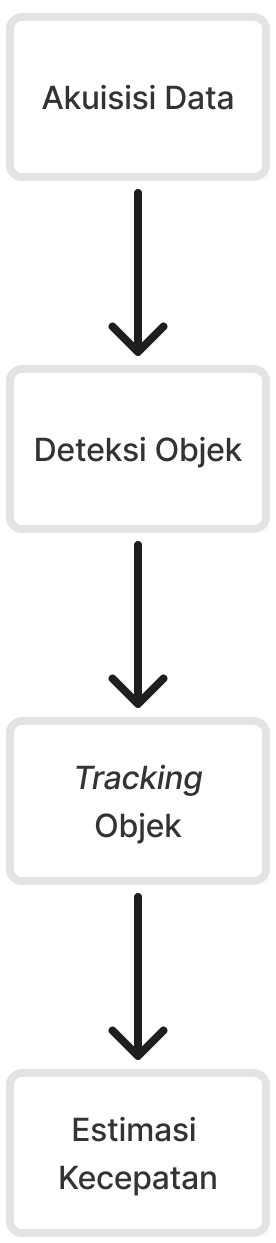
\includegraphics[width=0.1\textwidth]{gambar/diagramsistem.jpg}
    \caption{System workflow diagram.}
    \label{fig:system-arch}
\end{figure}

\subsection{Video Acquisition and Annotation}

Video is acquired using a DJI Phantom 4 Pro drone at various altitudes and lighting conditions. Annotation is conducted on Roboflow to prepare the dataset for training the YOLOv8 model.

\begin{figure}[H]
    \centering
    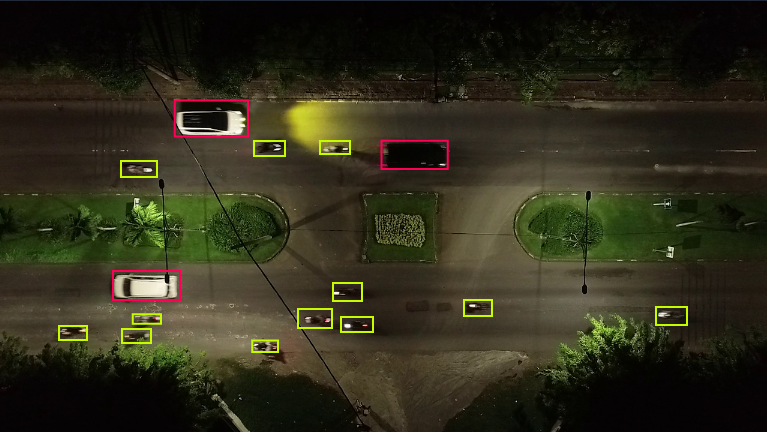
\includegraphics[width=0.45\textwidth]{gambar/anotasidatamalam.png}
    \caption{Example of annotated dataset (night).}
    \label{fig:annot-night}
\end{figure}

\begin{figure}[H]
    \centering
    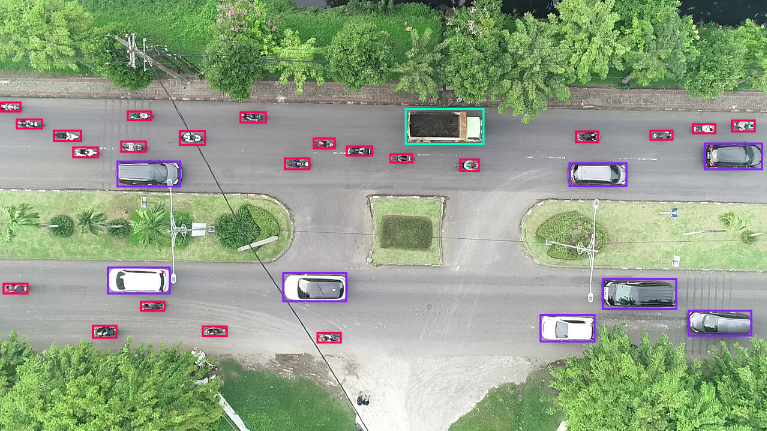
\includegraphics[width=0.45\textwidth]{gambar/anotasidatasiang.png}
    \caption{Example of annotated dataset (day).}
    \label{fig:annot-day}
\end{figure}

\subsection{Object Detection with YOLOv8-TensorRT}

Object detection is performed on video frames captured by a DJI Phantom 4 Pro drone, configured to record at a resolution of 720p and 30 FPS. The live video is transmitted to the Jetson Nano via RTMP streaming protocol, where real-time object detection is executed using a YOLOv8 model that has been converted into TensorRT format for efficient inference.

To reduce the processing load on the Jetson Nano, the video resolution is downscaled to 360p before inference. The YOLOv8 model has been trained to detect specific vehicle classes including cars, motorcycles, and trucks. Upon detection, each object is labeled and enclosed within a bounding box according to its classification.

The detection model only processes objects with a confidence threshold above 0.45, and bounding boxes are rendered for objects exceeding this threshold. Figure \ref{fig:deteksiobjek} shows an example of successful object detection on video frames using YOLOv8 in TensorRT format.

\begin{figure}[H]
    \centering
    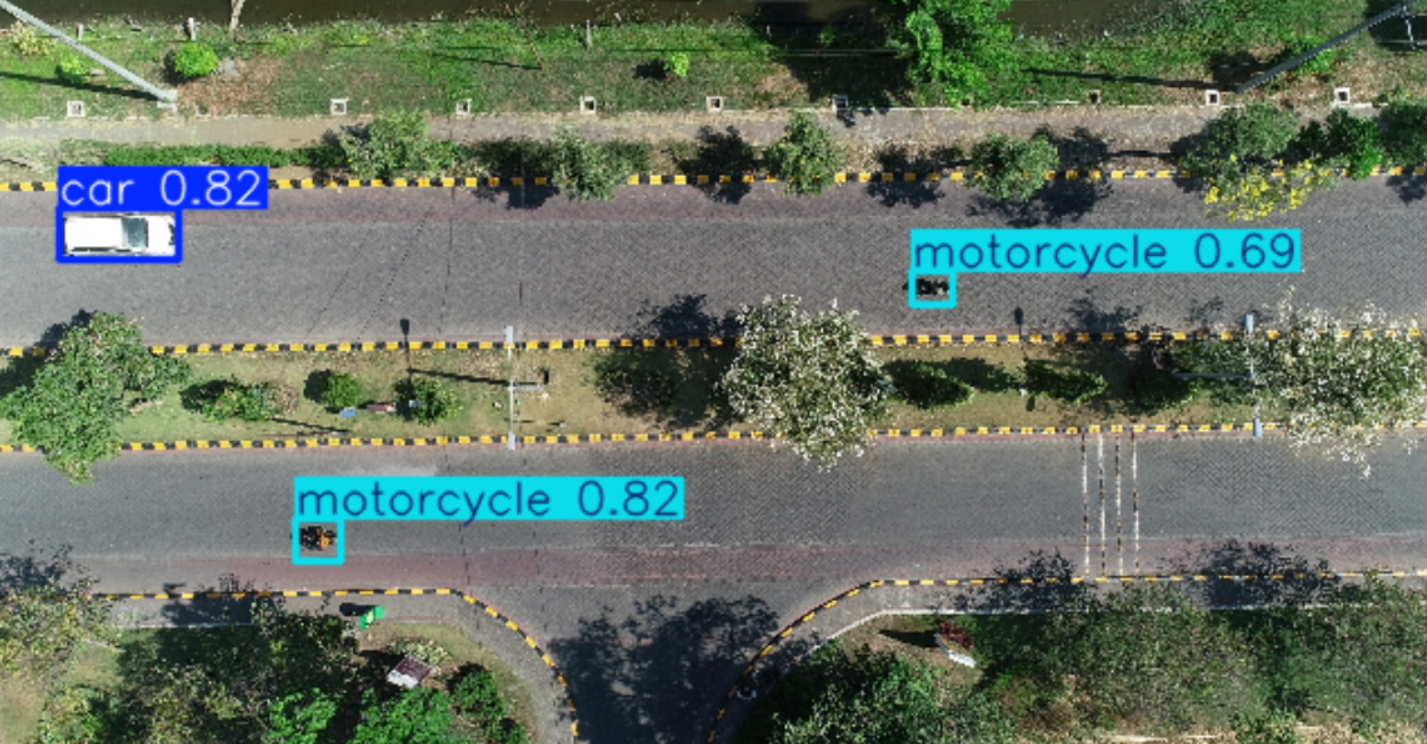
\includegraphics[width=0.45\textwidth]{gambar/deteksiobjek.png}
    \caption{Object detection output using YOLOv8 with TensorRT.}
    \label{fig:deteksiobjek}
\end{figure}


\subsection{Object Tracking with OC-SORT}

After vehicle objects are detected in each frame, tracking is employed to maintain object identity across successive frames. Two tracking algorithms were considered in this study: OC-SORT and ByteTrack.

Experimental results showed a notable difference between the two methods. ByteTrack offers faster processing speed, but at the cost of reduced tracking accuracy. In particular, ByteTrack occasionally fails to consistently assign bounding boxes to all detected objects, leading to incomplete tracking information.

Due to these limitations, this system utilizes the OC-SORT (Observation-Centric SORT) algorithm for object tracking. OC-SORT maintains better temporal consistency in assigning IDs to objects and performs well in aerial imagery scenarios where consistent motion patterns and occlusions are common.

To identify tracked objects uniquely, the center point of each bounding box is calculated using geometric midpoint formulas. This center is defined by:

\begin{equation}
    x_c = \frac{x_{min} + x_{max}}{2}, \quad
    y_c = \frac{y_{min} + y_{max}}{2}
\end{equation}

where $(x_{min}, y_{min})$ and $(x_{max}, y_{max})$ are the top-left and bottom-right coordinates of the bounding box. Each object is assigned a unique tracking ID along with its detected class label, allowing consistent tracking over time.

\subsection{Speed Estimation Process}

Once the objects are detected and tracked across frames, the system proceeds to estimate their speed. The movement of each object is calculated based on the displacement of its center point across frames using the Euclidean distance formula:

\begin{equation}
\label{eq:euclidean}
d = \sqrt{(x_2 - x_1)^2 + (y_2 - y_1)^2}
\end{equation}

where $(x_1, y_1)$ and $(x_2, y_2)$ represent the center coordinates of an object in two consecutive frames. This pixel-based displacement is then converted to meters using a scale factor derived from the Ground Sampling Distance (GSD) or Pixels per Meter (PPM), as shown in Table~\ref{tbl:skala_ppm}.

\begin{table}[H]
\centering
\caption{Meter-per-pixel scale based on drone altitude}
\label{tbl:skala_ppm}
\begin{tabular}{|c|c|}
\hline
\textbf{Altitude (m)} & \textbf{Meter per Pixel} \\ \hline
20 & 1 : 21.44 \\ \hline
30 & 1 : 14.30 \\ \hline
40 & 1 : 10.72 \\ \hline
\end{tabular}
\end{table}

To compute the object’s speed in kilometers per hour (km/h), the system applies the following equation:

\begin{equation}
\label{eq:speed_ms}
v = \frac{d}{t} \times 3.6
\end{equation}

where $d$ is the real-world displacement in meters (converted from pixels), $t$ is the time interval in seconds between frames, and $v$ is the estimated speed in km/h. The multiplier 3.6 converts speed from meters per second (m/s) to kilometers per hour (km/h), as commonly used in vehicle speedometers.

This method enables the system to estimate the vehicle's speed solely based on visual information from drone footage, making it suitable for flexible, infrastructure-free deployment.

\subsection{Streaming Setup}

The computation platform used in this study is the NVIDIA Jetson Nano, which acts as an edge device for running the detection, tracking, and speed estimation processes. The drone (DJI Phantom 4 Pro) transmits video streams via the Real-Time Messaging Protocol (RTMP). A shared network is established to ensure that the Jetson Nano is able to access the stream through a consistent IP configuration.

An RTMP server is configured using MediaMTX on a laptop. The drone sends its video feed to this server, and the Jetson Nano pulls the stream using FFmpeg integrated with OpenCV. The data transmission flow is illustrated in Figure~\ref{fig:alurdata}.

\begin{figure}[H]
    \centering
    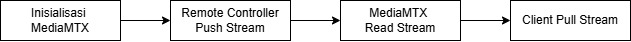
\includegraphics[width=0.45\textwidth]{gambar/pengirimandata.jpg}
    \caption{RTMP-based data transmission flow using MediaMTX.}
    \label{fig:alurdata}
\end{figure}

As shown in Figure~\ref{fig:alurdata}, the MediaMTX server is initialized on the laptop, and all devices are configured within the same local network. The Jetson Nano operates as the RTMP client, enabling it to receive and process the real-time video stream.

\subsection{System Processing Flow}

The core algorithm of the speed estimation program consists of several sequential stages, including frame acquisition, detection, tracking, and estimation. These components are implemented using a multithreaded pipeline for performance optimization. The processing flow of the system is illustrated in Figure~\ref{fig:diagramproses}.

\begin{figure}[H]
    \centering
    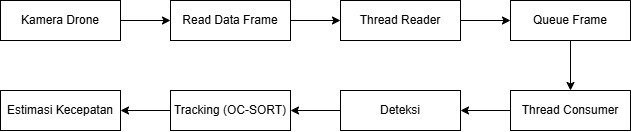
\includegraphics[width=0.45\textwidth]{gambar/algoritma.jpg}
    \caption{Program workflow for detection, tracking, and speed estimation.}
    \label{fig:diagramproses}
\end{figure}

\subsection{Hardware Topology}

The hardware configuration consists of the drone, a smartphone for controller interface, a laptop as the RTMP server, and the Jetson Nano as the inference device. The complete hardware topology is illustrated in Figure~\ref{fig:topologihardware}.

\begin{figure}[H]
    \centering
    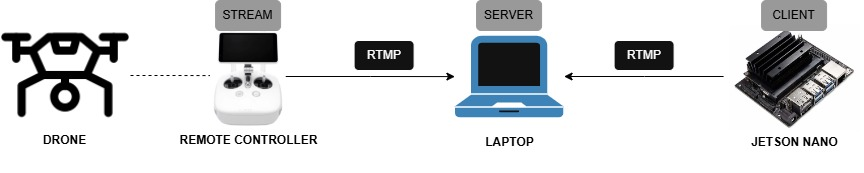
\includegraphics[width=0.45\textwidth]{gambar/topologi-hardware.jpg}
    \caption{Hardware topology for field deployment.}
    \label{fig:topologihardware}
\end{figure}

As shown in Figure~\ref{fig:topologihardware}, the RTMP protocol plays a central role in linking the drone's video feed to the Jetson Nano, enabling direct video input for on-site inference. This configuration allows for portable, real-time processing and visualization.

\subsection{Platform Specification}

The final system is deployed on a Jetson Nano using Ubuntu OS, CUDA, TensorRT, OpenCV, and PyTorch. RTMP stream is handled with FFmpeg and processed using OpenCV.

\begin{table}[H]
\centering
\caption{Jetson Nano Specification}
\label{tab:jetson-specs}
\begin{tabular}{|l|l|}
\hline
\textbf{Component} & \textbf{Specification} \\ \hline
CPU & Quad-core ARM Cortex-A57 @ 1.43 GHz \\ \hline
GPU & 128-core Maxwell NVIDIA GPU \\ \hline
Memory & 4 GB LPDDR4 RAM \\ \hline
Storage & microSD card slot (supports up to 64 GB) \\ \hline
\end{tabular}
\end{table}


\subsection{Vehicle Detection Model Evaluation}

Two YOLOv8 models were developed for object detection under different lighting conditions: daytime and nighttime. This section presents the training results, accuracy metrics, and validation outcomes for each model.

\subsubsection{Daytime Model Training Results}

The YOLOv8 model was trained using images captured during daylight over 250 epochs. Key metrics such as precision, recall, and mAP50 were recorded at selected checkpoints, as shown in Table~\ref{table:akurasi_model_siang}.

\begin{table}[H]
\caption{Training Accuracy of Daytime Detection Model}
\label{table:akurasi_model_siang}
\centering
\begin{tabular}{|c|c|c|c|}
\hline
\textbf{Epochs} & \textbf{Precision} & \textbf{Recall} & \textbf{mAP50} \\ \hline
50 & 0.67893 & 0.68114 & 0.6863 \\ \hline
100 & 0.76356 & 0.77383 & 0.72166 \\ \hline
160 (best) & 0.80555 & 0.79315 & 0.82471 \\ \hline
200 & 0.79412 & 0.76758 & 0.77683 \\ \hline
250 & 0.79412 & 0.76758 & 0.77683 \\ \hline
\end{tabular}
\end{table}

Figure~\ref{fig:grafik_model_siang} illustrates the training curves for bounding box loss, classification loss, and average precision.

\begin{figure}[H]
\centering
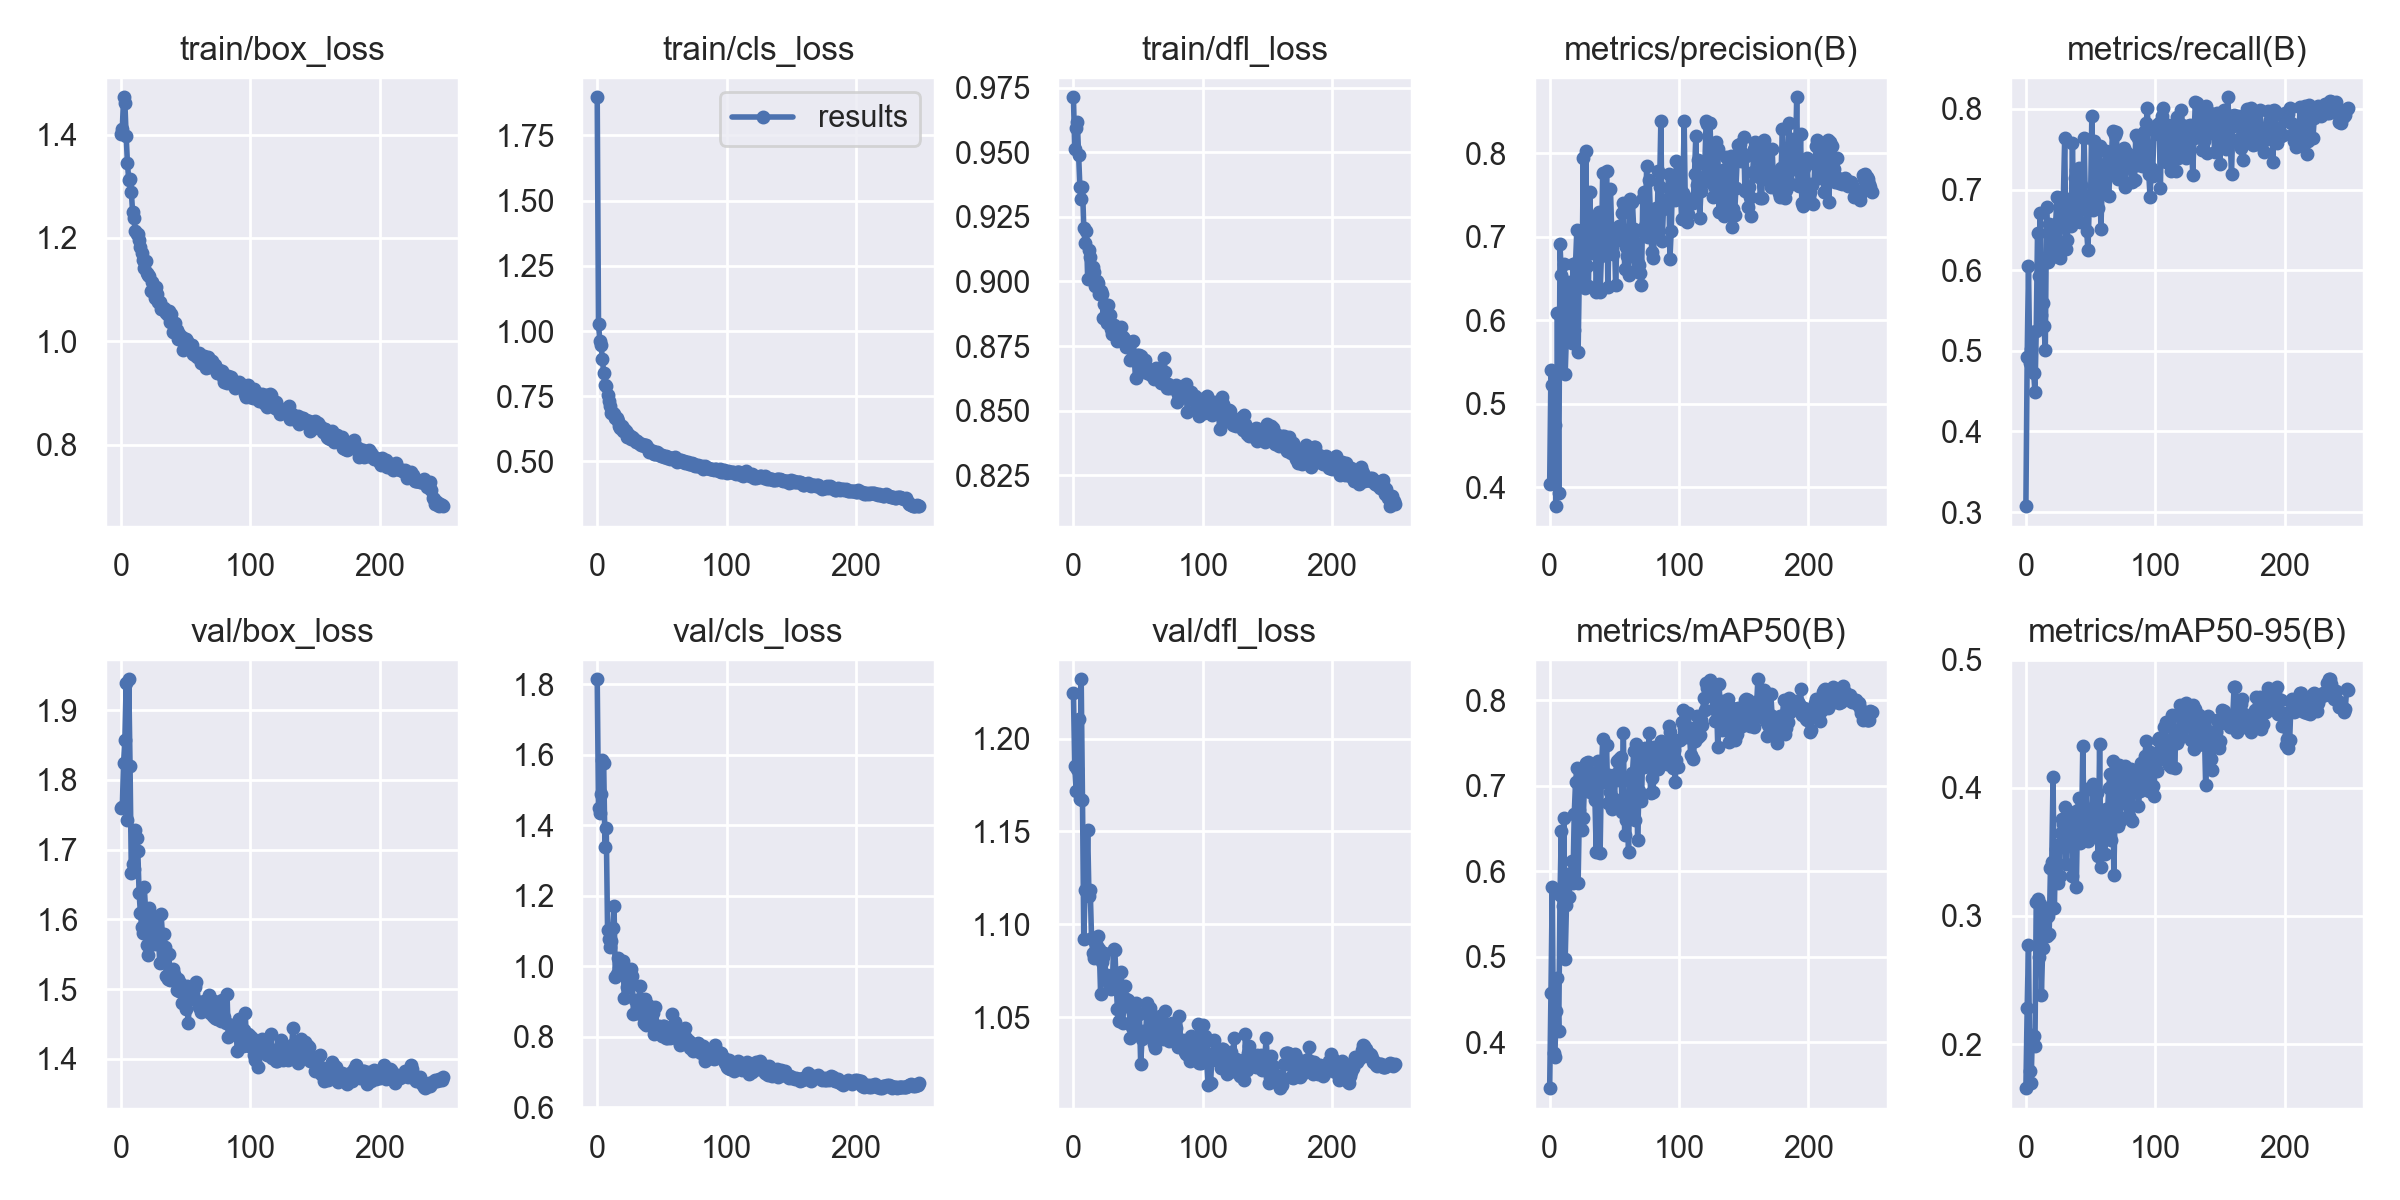
\includegraphics[width=0.45\textwidth]{gambar/results_siang.png}
\caption{Training curves for the daytime YOLOv8 model.}
\label{fig:grafik_model_siang}
\end{figure}

The confusion matrix in Figure~\ref{fig:confusion_matrix_siang} shows classification accuracy across object categories: car, motorcycle, truck, and background.

\begin{figure}[H]
\centering
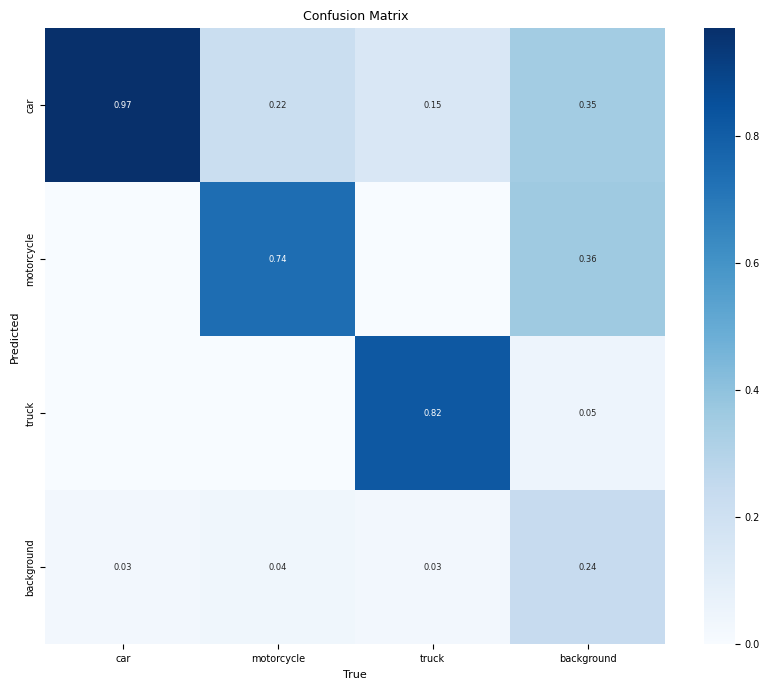
\includegraphics[width=0.45\textwidth]{gambar/confusion_siang.png}
\caption{Confusion matrix of the daytime detection model.}
\label{fig:confusion_matrix_siang}
\end{figure}

\begin{itemize}
    \item \textbf{Car:} 97\% correctly classified; minor confusion with background.
    \item \textbf{Motorcycle:} 74\% correct; 22\% misclassified as car.
    \item \textbf{Truck:} 82\% correct; minor confusion with background and car.
    \item \textbf{Background:} Model struggled, with frequent misclassification.
\end{itemize}

Validation results in Figure~\ref{fig:validasi_siang} show bounding boxes with confidence scores above 0.5.

\begin{figure}[H]
\centering
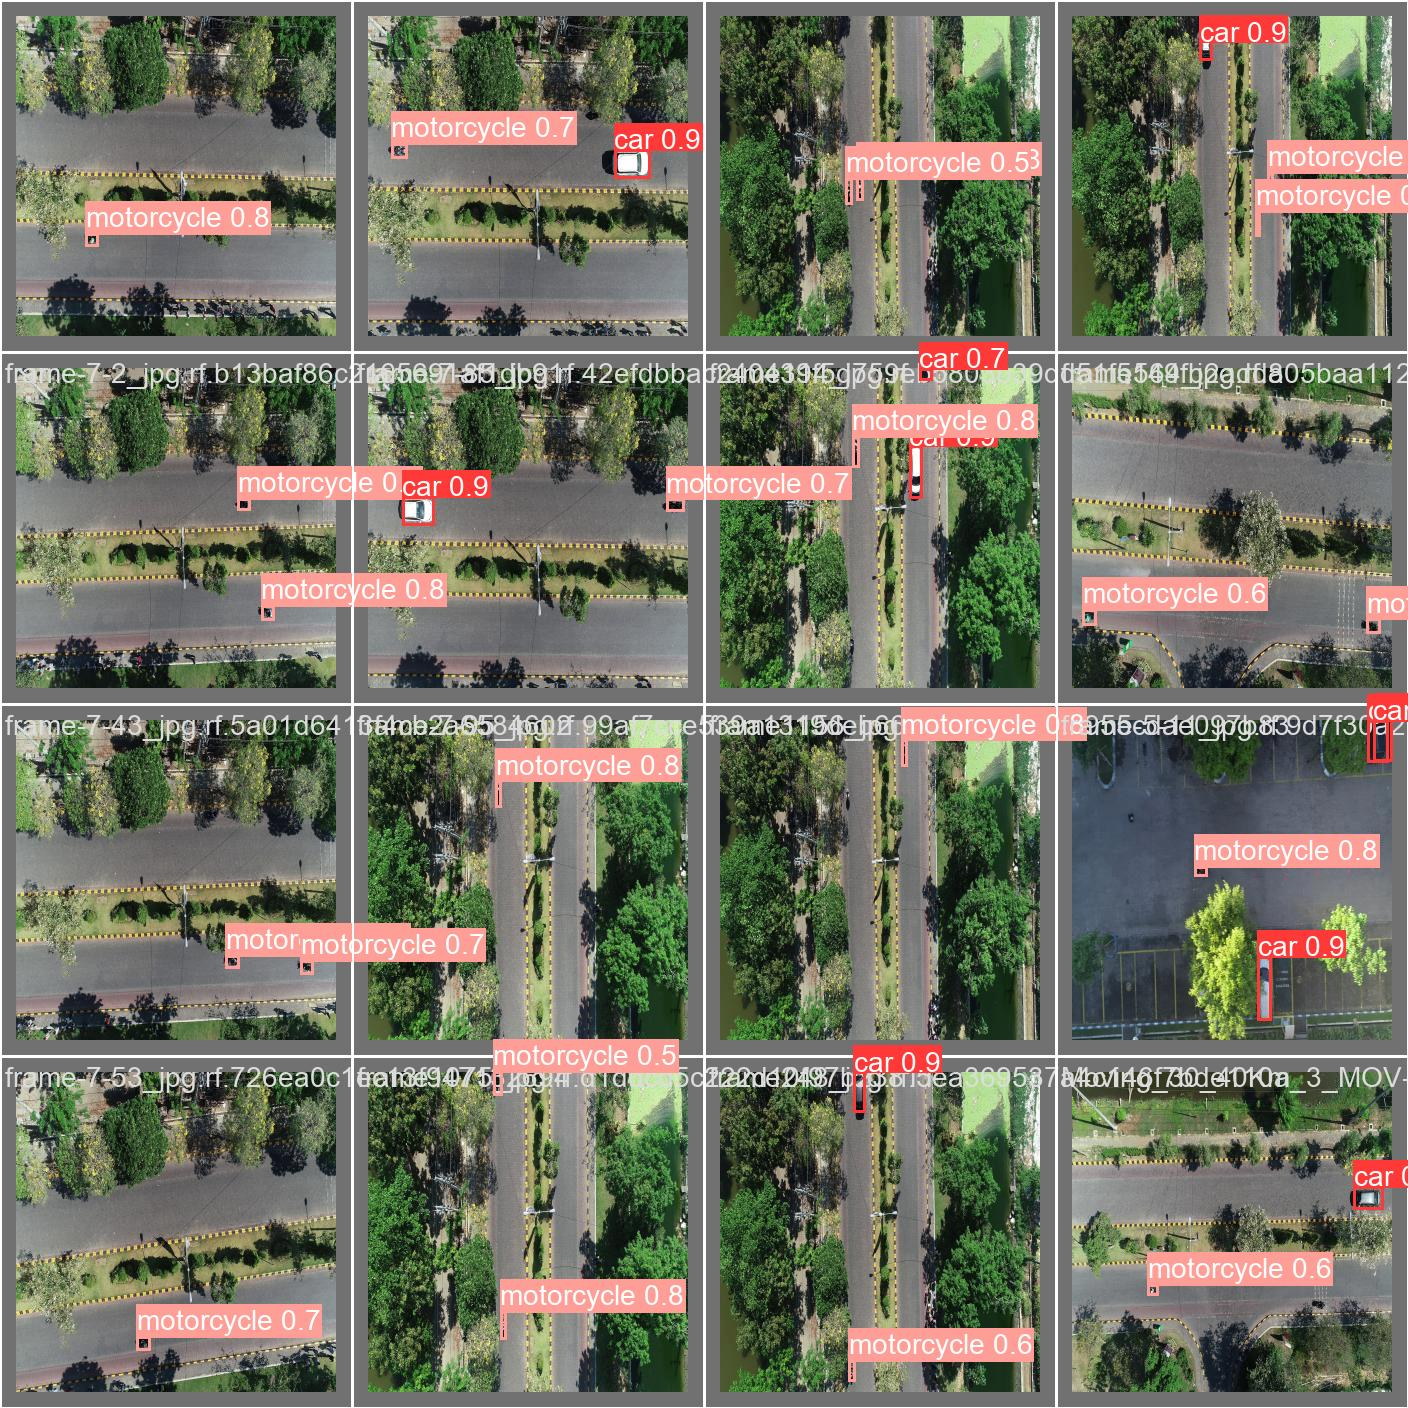
\includegraphics[width=0.45\textwidth]{gambar/val_batch_siang.jpg}
\caption{Validation results for the daytime model.}
\label{fig:validasi_siang}
\end{figure}

\subsubsection{Nighttime Model Training Results}

The nighttime model was trained on a low-light dataset for 250 epochs. Performance metrics are summarized in Table~\ref{table:akurasi_model_malam}.

\begin{table}[H]
\caption{Training Accuracy of Nighttime Detection Model}
\label{table:akurasi_model_malam}
\centering
\begin{tabular}{|c|c|c|c|}
\hline
\textbf{Epochs} & \textbf{Precision} & \textbf{Recall} & \textbf{mAP50} \\ \hline
50 & 0.81247 & 0.8977 & 0.81938 \\ \hline
72 (best) & 0.94688 & 0.88395 & 0.92997 \\ \hline
100 & 0.95264 & 0.88435 & 0.90664 \\ \hline
200 & 0.9409 & 0.89202 & 0.90600 \\ \hline
250 & 0.92616 & 0.88637 & 0.88913 \\ \hline
\end{tabular}
\end{table}

The training graphs in Figure~\ref{fig:grafik_model_malam} show steady improvements in both loss functions and detection metrics.

\begin{figure}[H]
\centering
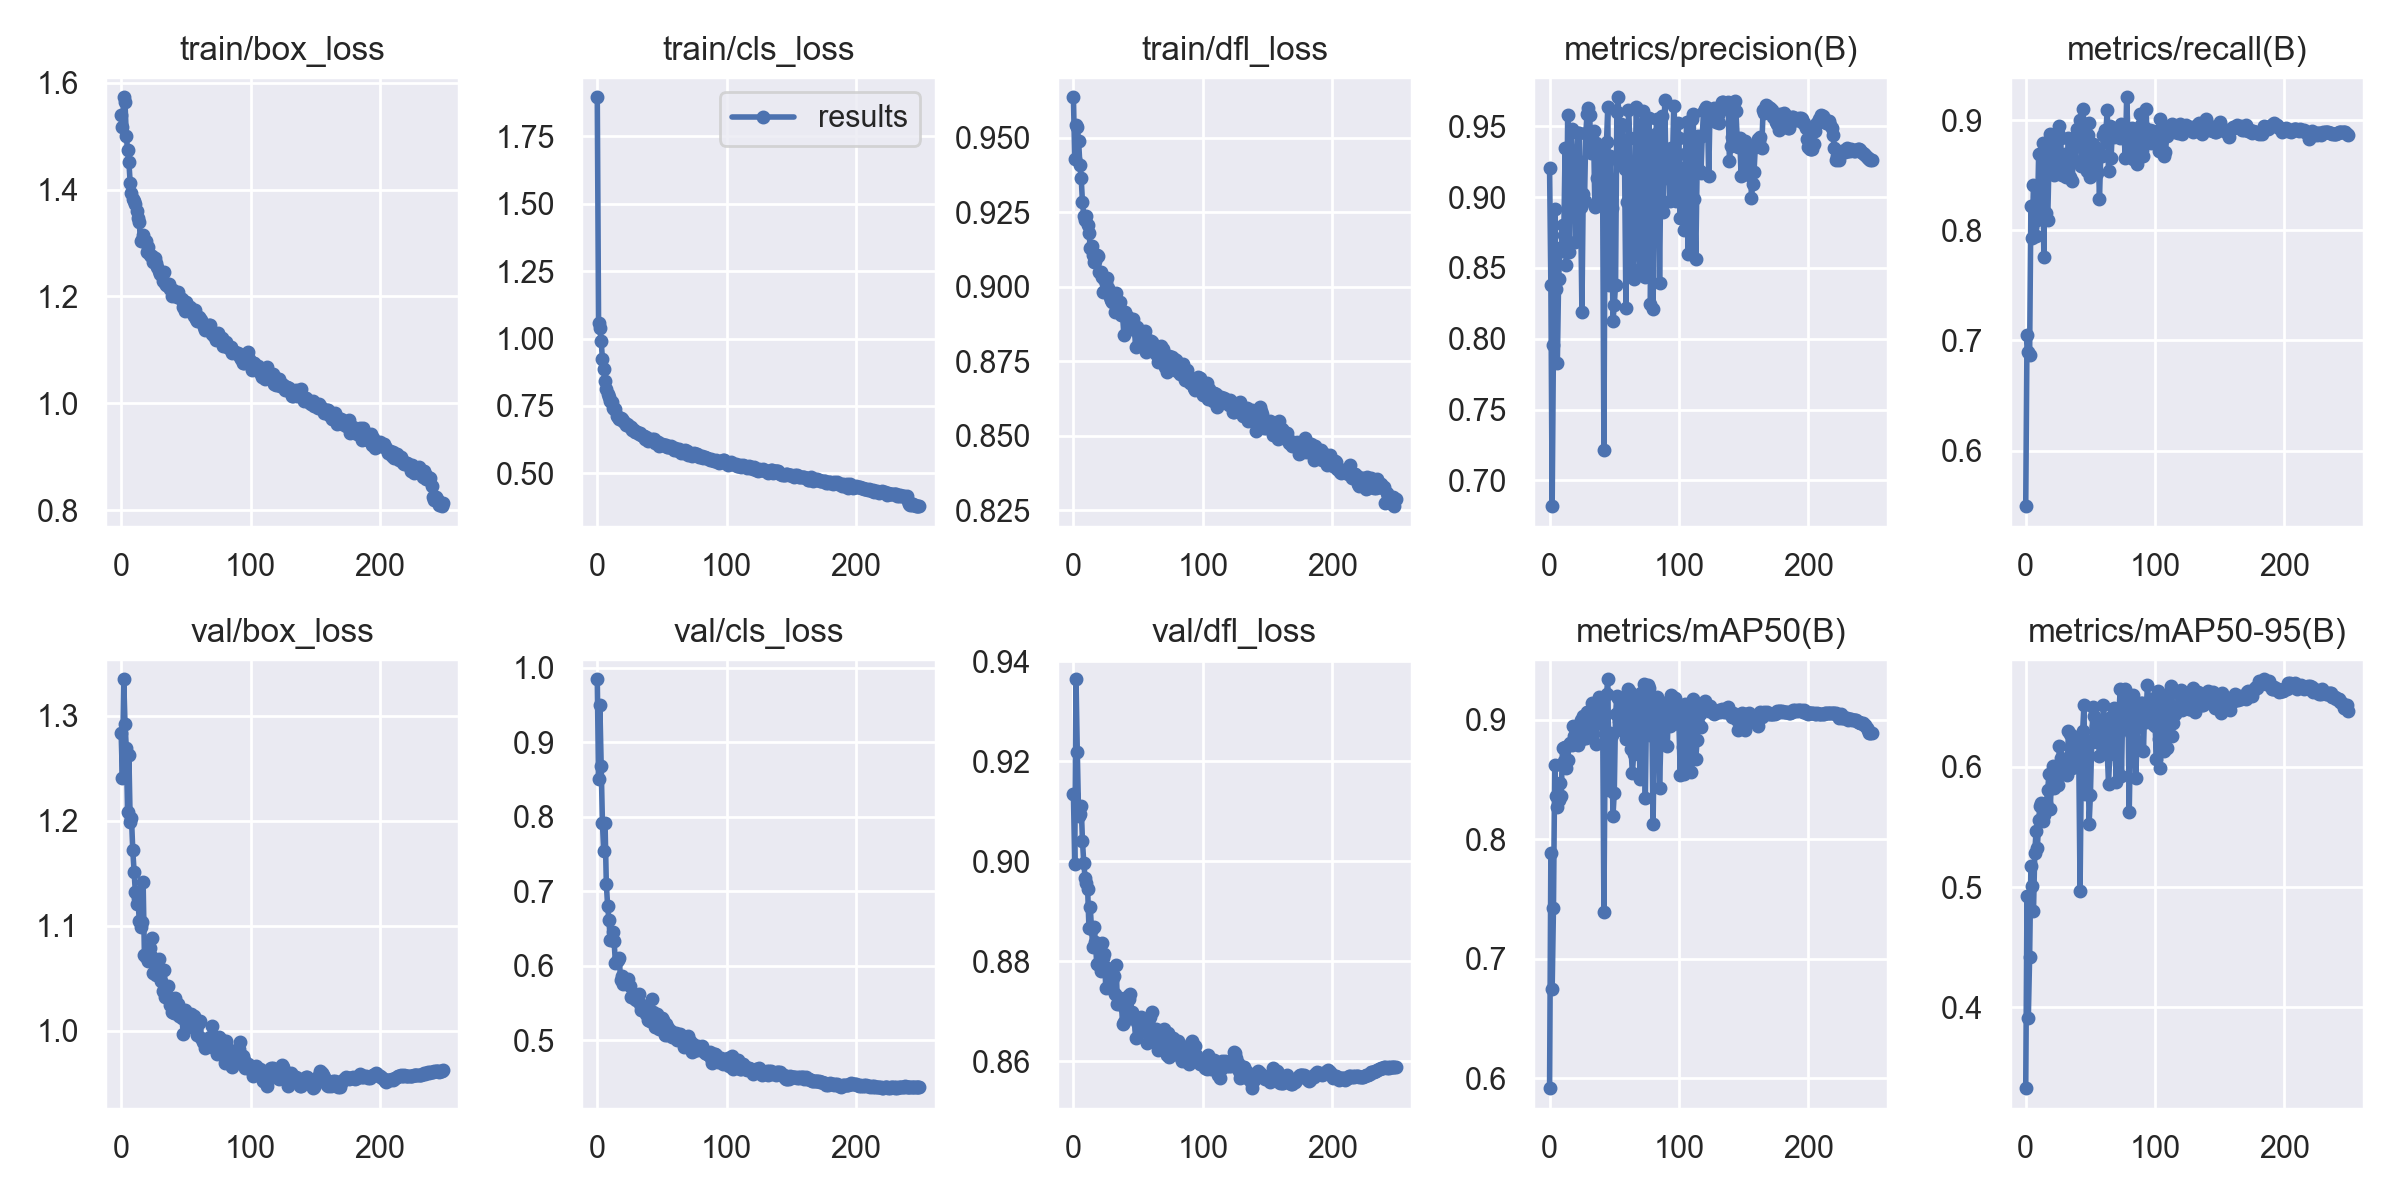
\includegraphics[width=0.45\textwidth]{gambar/grafik_model_malam.png}
\caption{Training curves for the nighttime YOLOv8 model.}
\label{fig:grafik_model_malam}
\end{figure}

Figure~\ref{fig:confusion_matrix_malam} shows the confusion matrix from the nighttime training run.

\begin{figure}[H]
\centering
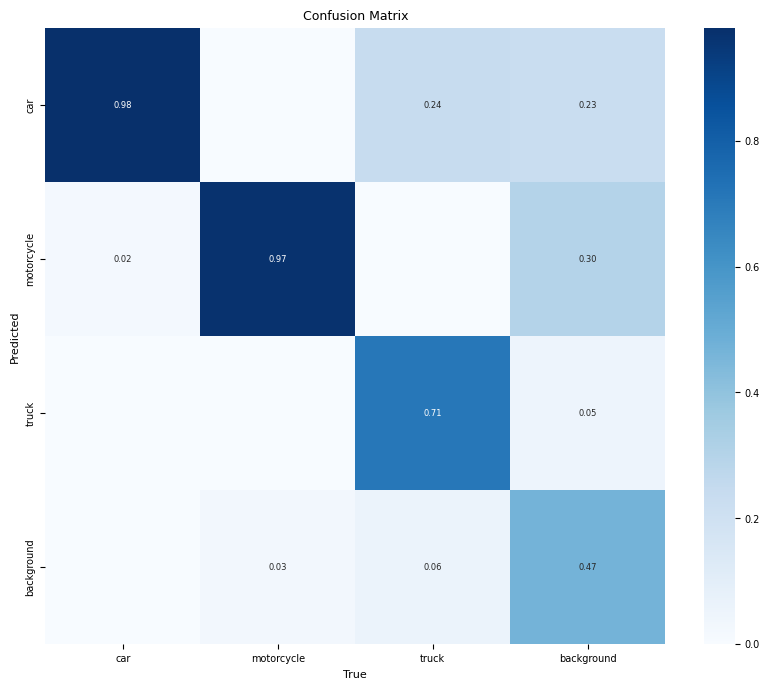
\includegraphics[width=0.45\textwidth]{gambar/confusion_malam.png}
\caption{Confusion matrix of the nighttime detection model.}
\label{fig:confusion_matrix_malam}
\end{figure}

\begin{itemize}
    \item \textbf{Car:} 98\% correct; 2\% misclassified as motorcycle.
    \item \textbf{Motorcycle:} 97\% correct; 3\% predicted as background.
    \item \textbf{Truck:} 71\% correct; 24\% misclassified as car.
    \item \textbf{Background:} Only 47\% correctly identified.
\end{itemize}

Validation results in Figure~\ref{fig:validasi_malam} indicate that smaller objects (motorcycles) yielded lower confidence values (min. 0.5) compared to larger ones (cars, up to 0.9).

\begin{figure}[H]
\centering
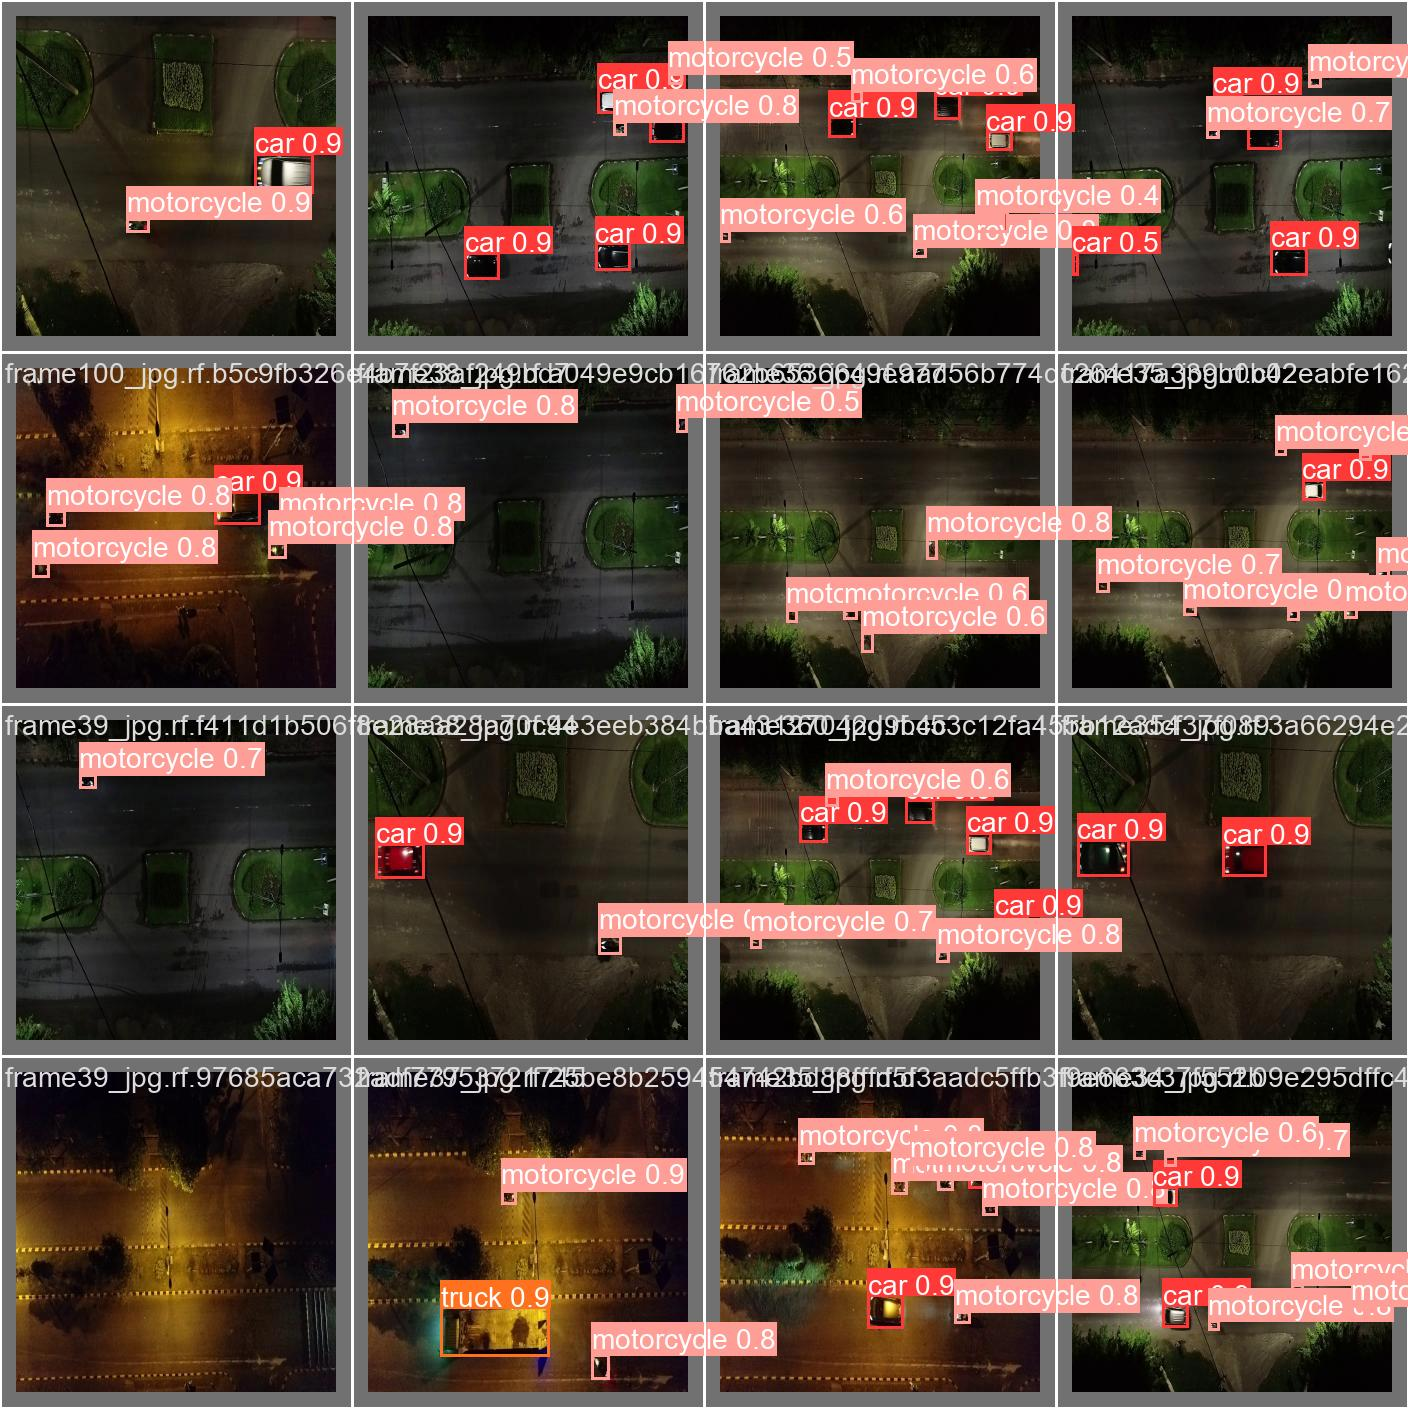
\includegraphics[width=0.45\textwidth]{gambar/val_batch_malam.jpg}
\caption{Validation results for the nighttime model.}
\label{fig:validasi_malam}
\end{figure}

\subsection{Comparison and Evaluation at 20 km/h in Daylight}

This subsection evaluates the system's speed estimation performance at a vehicle speed of 20 km/h in daylight conditions, and compares the results with prior research by Fatchurozi (2024) and Tilon \& Nex (2023).

Experiments were conducted with a motorcycle moving at an average speed of 20 km/h. The drone remained static at altitudes of 20 m, 30 m, and 40 m. Table~\ref{table:manual_speed_calc} shows the manually measured average speed.

\begin{table}[htbp]
\centering
\caption{Manual Speed Calculation at 20 km/h}
\label{table:manual_speed_calc}
\begin{tabular}{|c|c|c|c|c|}
\hline
\textbf{Altitude (m)} & Run 1 & Run 2 & Run 3 & \textbf{Average (km/h)} \\ \hline
20 & 23.33 & 22.90 & 22.30 & 22.84 \\ \hline
30 & 18.94 & 18.80 & 18.76 & 18.83 \\ \hline
40 & 18.81 & 18.79 & 18.72 & 18.77 \\ \hline
\end{tabular}
\end{table}

Table~\ref{table:system_speed_calc} presents the results of the proposed system, including mean and standard deviation.

\begin{table}[htbp]
\centering
\caption{Speed Estimation by Proposed System at 20 km/h}
\label{table:system_speed_calc}
\begin{tabular}{|c|c|c|c|c|c|}
\hline
\textbf{Altitude (m)} & Run 1 & Run 2 & Run 3 & \textbf{Average} & \textbf{Std. Dev.} \\ \hline
20 & 21.59 & 20.06 & 21.61 & 21.09 & 0.72 \\ \hline
30 & 23.28 & 21.25 & 25.05 & 23.19 & 1.55 \\ \hline
40 & 22.24 & 24.39 & 21.70 & 22.78 & 1.16 \\ \hline
\end{tabular}
\end{table}

Error calculations for Trial 1 are shown in Table~\ref{table:error_accuracy_t1}.

\begin{table}[htbp]
\centering
\caption{Error and Accuracy - Trial 1}
\label{table:error_accuracy_t1}
\begin{tabular}{|c|c|c|c|c|}
\hline
\textbf{Altitude (m)} & Error & Absolute Error & Relative Error (\%) & Accuracy (\%) \\ \hline
20 & -1.74 & 1.74 & 7.46 & 92.54 \\ \hline
30 & 4.34 & 4.34 & 22.91 & 77.09 \\ \hline
40 & 3.43 & 3.43 & 18.23 & 81.77 \\ \hline
\end{tabular}
\end{table}

The system showed the highest accuracy at 20 m altitude across all trials. At higher altitudes, reduced pixel density lowered speed estimation accuracy.

Table~\ref{table:accuracy_fatchurozi} summarizes results from Fatchurozi (2024) for 20 km/h scenarios, while Table~\ref{table:accuracy_tilon} shows the accuracy from Tilon \& Nex (2023) at 15 km/h and 50 m altitude.

\begin{table}[htbp]
\centering
\caption{Accuracy Comparison with Fatchurozi (2024)}
\label{table:accuracy_fatchurozi}
\begin{tabular}{|c|c|c|c|}
\hline
\textbf{Altitude (m)} & Trial 1 (\%) & Trial 2 (\%) & Trial 3 (\%) \\ \hline
20 & 89.75 & 90.52 & 88.26 \\ \hline
30 & 93.47 & 91.55 & 87.98 \\ \hline
40 & 86.11 & 94.96 & 89.13 \\ \hline
\end{tabular}
\end{table}

\begin{table}[htbp]
\centering
\caption{Accuracy from Tilon \& Nex (2023) at 15 km/h}
\label{table:accuracy_tilon}
\begin{tabular}{|c|c|}
\hline
\textbf{Altitude (m)} & Accuracy (\%) \\ \hline
50 & 77.59 \\ \hline
\end{tabular}
\end{table}

The proposed system achieved accuracy exceeding 90\% at 20 m altitude, which decreased at higher altitudes. Compared to previous studies, the system performs competitively, particularly at low altitudes. Key influencing factors include altitude, image resolution, and vehicle type. Real-time edge processing on Jetson Nano enhances the system’s applicability in portable deployments.



% Ubah judul dan label berikut sesuai dengan yang diinginkan.
\section{Conclusion}
\label{sec:conclusion}

% Ubah paragraf-paragraf pada bagian ini sesuai dengan yang diinginkan.

This study developed a vehicle speed estimation system using a DJI Phantom 4 drone and YOLOv8 deep learning model, integrated with a Jetson Nano for edge processing. The system demonstrated its ability to detect vehicles and estimate their speed with reasonable accuracy in both daytime and nighttime conditions.

The results show that the system's accuracy in vehicle detection and speed estimation is affected by environmental factors, such as lighting conditions and altitude. During daytime, the model achieved a high mAP50 of 0.92997 at epoch 72, while nighttime testing showed slightly lower performance but still promising results. Speed estimation errors ranged from 10\% to 16.8\%, depending on the test conditions, with higher errors observed at higher speeds and greater altitudes.

The system's performance is limited by the hardware capabilities of the Jetson Nano, with a frame rate of 15 FPS and some latency in real-time processing. However, the system remains functional for low-speed vehicle detection and can be further optimized for higher accuracy and performance with improved hardware and software optimizations.

In conclusion, the proposed system is a promising solution for real-time traffic monitoring and speed estimation, especially in controlled environments. Future improvements, including hardware upgrades and further model fine-tuning, can enhance its accuracy and applicability in various real-world scenarios.

% Acknowledgment jika ada
\section{Acknowledgement}
\label{sec:acknowledgement}


% Menampilkan daftar pustaka dengan format IEEE
\bibliographystyle{IEEEtranN}
\bibliography{pustaka/pustaka.bib}

% Menyeimbangkan bagian akhir di kedua kolom
\balance

\end{document}
